\documentclass{beamer}
\usepackage[utf8]{inputenc}
\usepackage{graphicx}
\usepackage{color}
%\usetheme{Hannover}
\newcommand{\hilight}[1]{\textbf{\textcolor{structure.fg!85}{#1}}}
\setbeamertemplate{footline}[frame number]

\usepackage{hyperref}
\hypersetup{
    colorlinks=true,
    linkcolor=blue,
    filecolor=magenta,      
    urlcolor=cyan,
}

\author[Sowmya Vajjala]{Sowmya Vajjala}

\title[SfSNLP]{NLP without Annotated Dataset}
\subtitle{Building a Spam Classifier with Snorkel}


\date{18 January 2021}

\institute{Seminar f\"ur Sprachwissenschaft, University of T\"ubingen, Germany}
%%%%%%%%%%%%%%%%%%%%%%%%%%%

\begin{document}

\begin{frame}\titlepage
\end{frame}

\begin{frame}{Class Outline}
    \begin{itemize}
        \item Generating training data for youtube spam classification
        \begin{enumerate}
            \item Using labeling functions
            \item Using transformation functions
        \end{enumerate}
        \item Training a classifier, and seeing how it does
        \item Assignment 2 Description
    \end{itemize}
    \small Note: Today's class heavily relies on \href{https://github.com/snorkel-team/snorkel-tutorials/tree/master/spam}{Snorkel's official spam classification tutorial}. I did not upload my code yet - will do tonight or tomorrow after cleaning it up a little bit. 
    
    \small note: This is a long session staring at and discussing code snippets/screenshots. Take a deep breath!
\end{frame}

\begin{frame}
\frametitle{Term papers schedule}
\begin{itemize}
\item We are starting this Friday!
    \item Teams/Papers info on the forum.
    \item Presentation schedule  (also posted on forum)
    \begin{enumerate}
        \item 22nd January: Teams 1--3
        \item 25th January: Teams 4--7
        \item 27th January: Teams 7--9
    \end{enumerate}
    \item Format: 15-20 minutes of presentation, Around 10 min of discussion per team (everyone can ask questions. Presenters don't have to know all answers. I will also try to answer some of the questions that come up!)
\end{itemize}
Questions on this? 
\end{frame}

\begin{frame}
\frametitle{In the last class}
\begin{itemize}
    \item Anonymization of data in NLP 
    \item Generating your own data
        \begin{itemize}
    \item Weak supervision: An overview
    \item Automatic Data Labeling: Some examples
    \item Data Augmentation: Some examples
    \item Text classification: An overview
    \end{itemize}
-We will see how can data labeling and augmentation be used for text classification today.  Any questions so far?
\end{itemize}
\end{frame}


\begin{frame}{}
    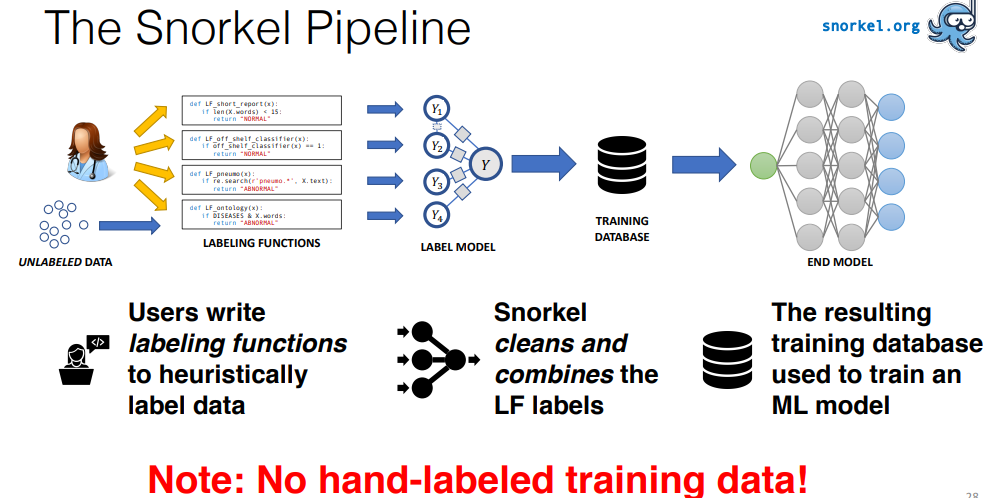
\includegraphics[width=\textwidth]{figures/snorkelradiologyexample.PNG}
    \href{Source}{https://db.cs.washington.edu/events/workshop/2019/slides/alex-ratner.pdf}
\end{frame}

\begin{frame}
\frametitle{How to "create" data?}
    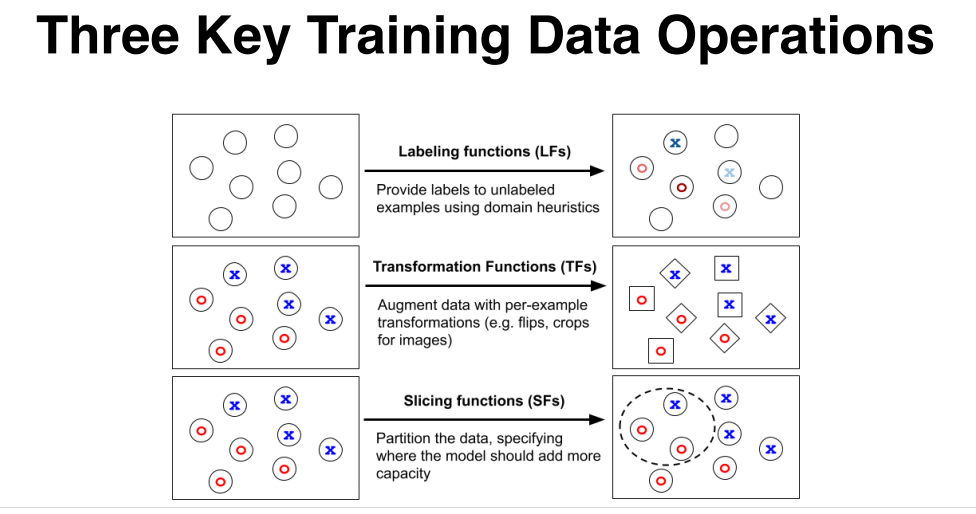
\includegraphics[width=\textwidth]{figures/3snorkelops.PNG}
\end{frame}

\begin{frame}
\frametitle{Source dataset}
    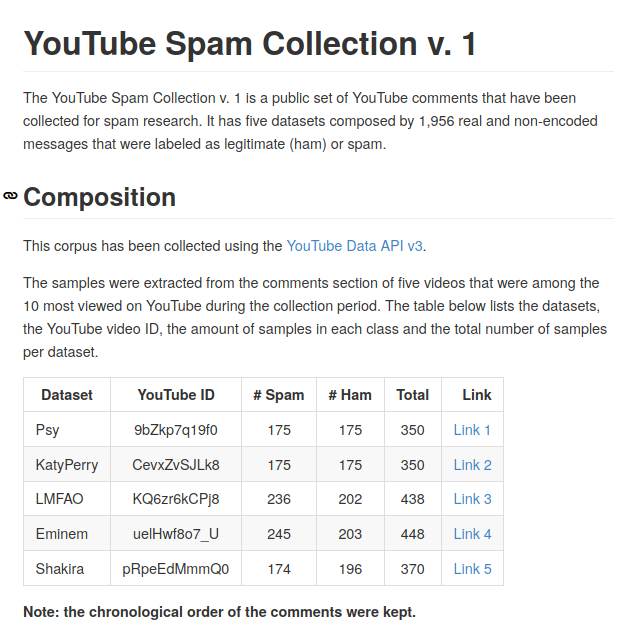
\includegraphics[width=0.7\textwidth]{figures/youtubedataset.png}
\end{frame}

\begin{frame}[fragile]
\frametitle{Source dataset}
\begin{itemize}
    \item The dataset contains comments from 5 of the most popular YouTube videos during a period between 2014 and 2015.
    \item The tutorial has some utility functions to load and explore their sample dataset. It has a load\_spam\_dataset() function that downloads the raw CSV files from the internet, divides them into splits, converts them into DataFrames, and shuffles them.
    \item  The first four videos' comments are combined to form the train set. This set has no gold labels. The fifth video is part of the test set.
\end{itemize}
\end{frame}

\begin{frame}{Loading the dataset}
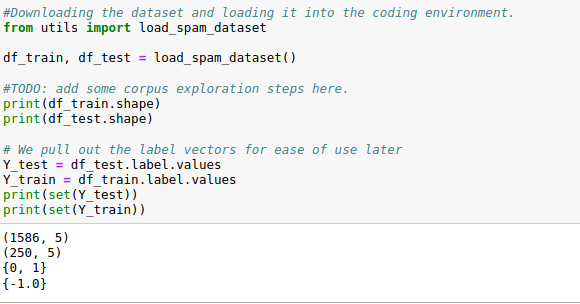
\includegraphics[width=\textwidth]{figures/loadingdatasnorkel.png}
Note: The dataset has label information. However, we are here not going to use training set labels. We will use test set labels to evaluate our approach. 
\end{frame}

\begin{frame}{}
    \Large Labeling Functions
\end{frame}

\begin{frame}{Labeling Functions}
    \begin{itemize}
        \item LFs are heuristics that take as input a data point and either assign a label to it (in this case, `HAM` or `SPAM`) or abstain (don't assign any label). \pause
        \item They are a way of encoding some domain knowledge or some other relevant information to generate training data programmatically. \pause
        \item Labeling functions can be *noisy*: they don't have perfect accuracy and don't have to label every data point.
        \item  Moreover, different labeling functions can overlap (label the same data point) and even conflict (assign different labels to the same data point).
    \end{itemize}
\end{frame}

\begin{frame}{They come in various forms}
\begin{enumerate}
    \item Keyword searches: looking for specific words in a sentence
    \item Pattern matching: looking for specific syntactical patterns
    \item Third-party models: using an pre-trained model (usually a model for a different task than the one at hand)
    \item Distant supervision: using external knowledge base
    \item Crowdworker labels: treating each crowdworker as a black-box function that assigns labels to subsets of the data
\end{enumerate} 
\end{frame}

\begin{frame}{How do we develop LFs?}
A typical LF development cycle consists of the following steps:
\begin{itemize}
    \item  Look at examples in training data to generate ideas for LFs
    \item  Write an initial version of an LF
    \item Check how this dose in terms of its coverage, overlap with other LFs etc.
    \item Improve the LF or look for a new LF by inspecting the data further
\end{itemize}
\end{frame}

\begin{frame}{Things to keep in mind}
    \begin{itemize}
        \item Our goal for LF development is to create a high quality set of training labels for our unlabeled dataset, not to label everything or directly create a model for inference using the LFs. \pause
        \item The training labels are used to train a separate discriminative model (in this case, one which just uses the comment text) in order to generalize to new, unseen data points. 
        \item Using this model, we can make predictions for data points that our LFs don't cover.
    \end{itemize}
\end{frame}

\begin{frame}
\frametitle{Exploring the dataset-1}
    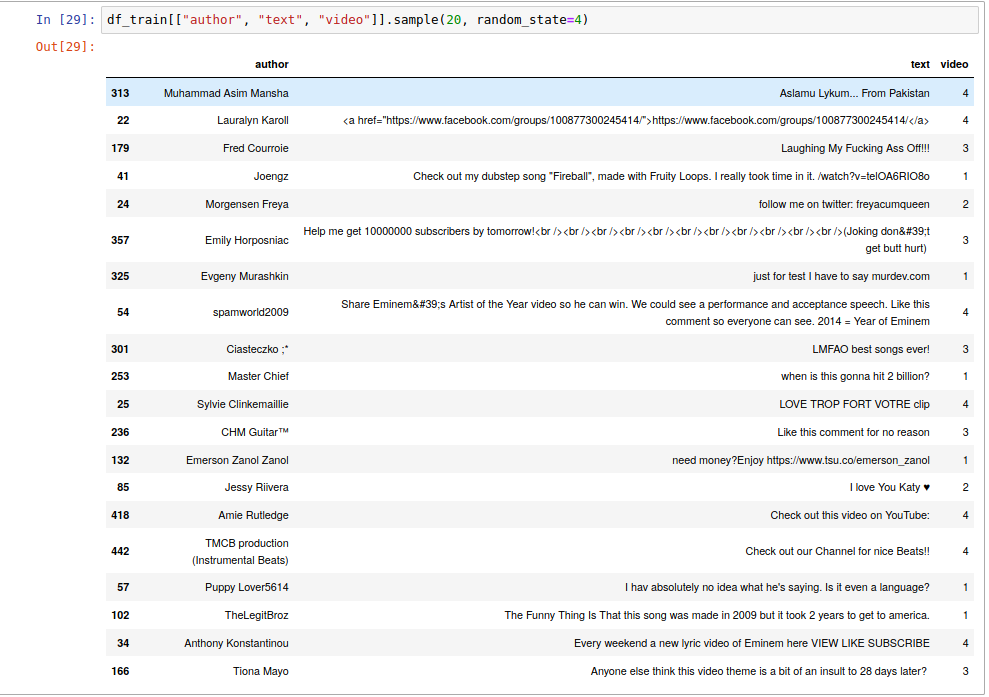
\includegraphics[width=0.9\textwidth]{figures/sample1.png}
\end{frame}

\begin{frame}
\frametitle{Exploring the dataset -2}
    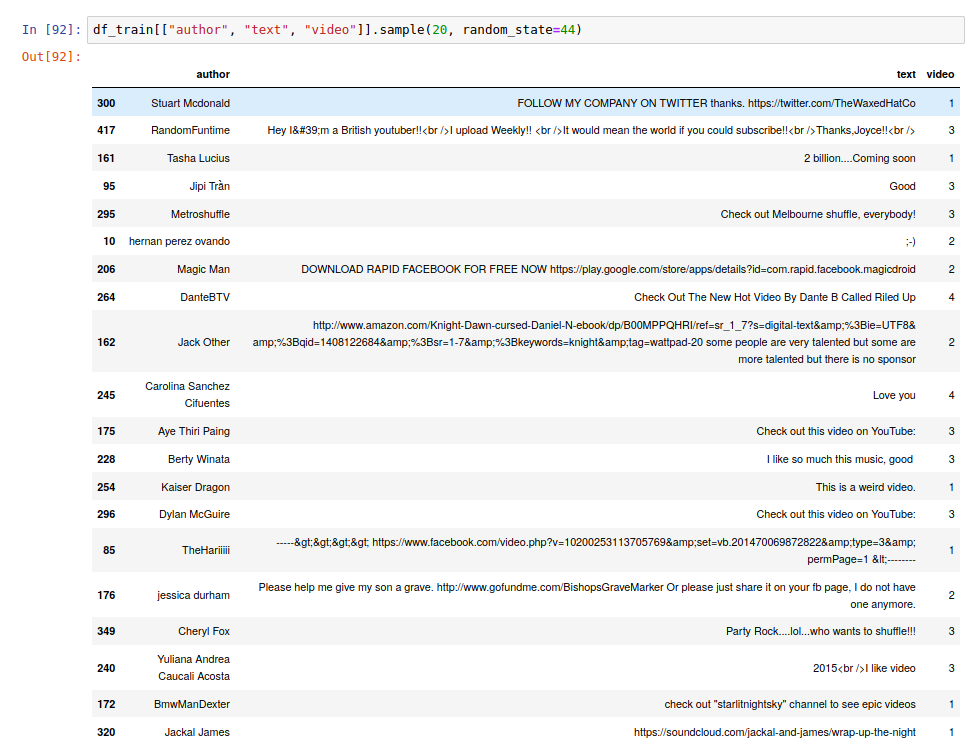
\includegraphics[width=0.9\textwidth]{figures/sample2.png}
\end{frame}

\begin{frame}{Before I start...}
Let us do a small exercise. Under today's class (Topic 5), there is a folder with csv files - which is our dataset. In these csv files, there are comments and their classification, and some meta data. Ignore all other columns, just look at comments text (don't cheat and look at labels!) and see if you can identify what is spam and what is not, and if there are any patterns to that and if you can design some LFs (you dont have to code. Just plan). Look at the file with your group/room number. 

Time: 20 minutes
    
\end{frame}

\begin{frame}{}
    \Large Share your observations
\end{frame}

\begin{frame}[fragile]
\frametitle{Some Keyword LFs for Spam category}
\small
\begin{verbatim}
from snorkel.labeling import labeling_function
@labeling_function()
def subscribe(x):
    return SPAM if "subscribe" in x.text.lower() else ABSTAIN

@labeling_function()
def help_me(x):
    return SPAM if "help" in x.text.lower() else ABSTAIN

@labeling_function()
def need_money(x):
    return SPAM if "money" in x.text.lower() else ABSTAIN

@labeling_function()
def http(x):
    return SPAM if "http" in x.text.lower() else ABSTAIN
\end{verbatim}
\end{frame}

\begin{frame}[fragile]
\frametitle{Some Keyword LFs for Ham category}
\small
\begin{verbatim}
@labeling_function()
def good(x):
    return HAM if "good" in x.text.lower() else ABSTAIN

@labeling_function()
def love(x):
    return HAM if "love" in x.text.lower() else ABSTAIN

@labeling_function()
def best(x):
    return HAM if "best" in x.text.lower() else ABSTAIN
\end{verbatim}
\end{frame}
%Mention how I was exploring functions - thank, need money vs money etc 

\begin{frame}[fragile]
\frametitle{Pattern based LF with regex}
\small
\begin{verbatim}
@labeling_function()
def check_out(x):
    return SPAM if re.search(r"check.*out", x.text, flags=re.I) else ABSTAIN
\end{verbatim}
\end{frame}

\begin{frame}[fragile]
\frametitle{Heuristics based LF}
\small
\begin{verbatim}
@labeling_function()
def short_comment(x):
    """Ham comments are often short, such as 'cool video!'"""
    return HAM if len(x.text.split()) < 5 else ABSTAIN
\end{verbatim}
\end{frame}

\begin{frame}[fragile]{LF with external tools}
    \small
\begin{verbatim}
#memoize option is to cache the output so that functions 
#that use this function don't have to rerun it each time. 
@preprocessor(memoize=True)
def textblob_sentiment(x):
    scores = TextBlob(x.text)
    x.polarity = scores.sentiment.polarity
    x.subjectivity = scores.sentiment.subjectivity
    return x

@labeling_function(pre=[textblob_sentiment])
def textblob_subjectivity(x):
    return HAM if x.subjectivity >= 0.5 else ABSTAIN
\end{verbatim}
\end{frame}

\begin{frame}[fragile]{LFs with more complex pre-processors}
\tiny
    \begin{verbatim}
from snorkel.preprocess.nlp import SpacyPreprocessor

# The SpacyPreprocessor parses the text in text_field and
# stores the new enriched representation in doc_field
spacy = SpacyPreprocessor(text_field="text", doc_field="doc", memoize=True)

@labeling_function(pre=[spacy])
def has_person(x):
    """Ham comments mention specific people and are short."""
    if len(x.doc) < 20 and any([ent.label_ == "PERSON" for ent in x.doc.ents]):
        return HAM
    else:
        return ABSTAIN

from snorkel.labeling.lf.nlp import nlp_labeling_function

@nlp_labeling_function()
def has_person_nlp(x):
    """Ham comments mention specific people and are short."""
    if len(x.doc) < 20 and any([ent.label_ == "PERSON" for ent in x.doc.ents]):
        return HAM
    else:
        return ABSTAIN

    \end{verbatim}
\end{frame}

\begin{frame}[fragile]{Do these LFs do anything?}
\framesubtitle{How many examples do they even cover?}
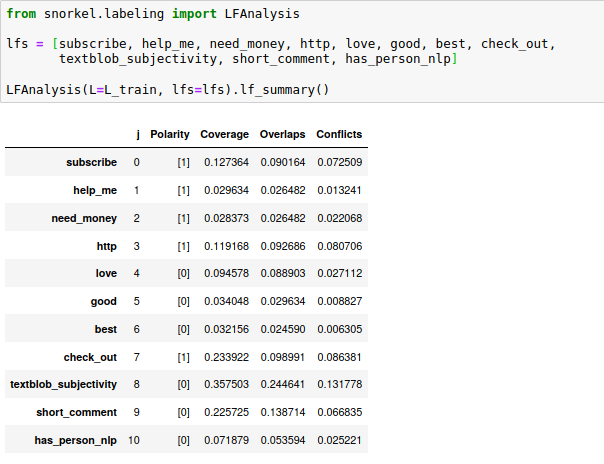
\includegraphics[width=\textwidth]{figures/lfanalysis.png}
\end{frame}

\begin{frame}{Coverage, Conflicts, FPs etc.}
At this point, it is a good idea to check some sample labeled output for each LF, to ensure it is not too off-track. 
    \begin{itemize}
        \item Coverage indicates how many examples in the training set does an LF cover.
        \item Conflicts indicate other LFs that reach a different categorization for a given LF.
        \item Overlaps indicate cases which are covered by at least one another LF. 
    \end{itemize}
We need good coverage, without too many conflicts, and without glaring false positives for an LF.
\end{frame}

\begin{frame}[fragile]{Applying LFs on the dataset}
\small
\begin{verbatim}
applier = PandasLFApplier(lfs=lfs)
L_train = applier.apply(df=df_train)
L_test = applier.apply(df=df_test)
\end{verbatim}
Since I have 11 LFs, each data point in train/test set is now a 11-dimensional vector, each dimension indicating an LF's decision for it. 
\end{frame}

\begin{frame}{Choosing among LFs}
    \begin{itemize}
        \item Some of these LFs may just be overlapping a lot, or getting a lot of false positives or just too infrequent. How do we check for these?
        \item How do we compare the outputs of two LFs for a single (or a couple of data instances?)
        \item Snorkel has some built in tools for running this kind of analyses (note: I did not run these analyses!)
        \item There are also several other plotting tools (see the full snorkel tutorial for details) to do various analyses on LFs and their results. 
    \end{itemize}
\end{frame}

\begin{frame}[fragile]{LFs analysis - 1}
\framesubtitle{How good is an LF?}
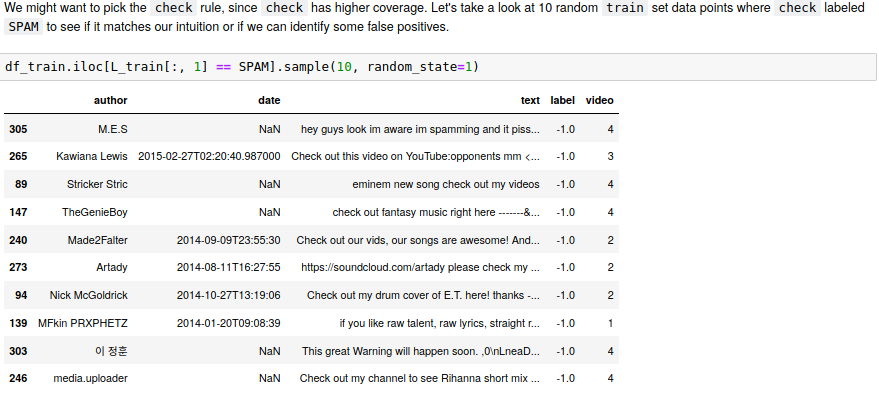
\includegraphics[width=\textwidth]{figures/examplelfanalysis1.png}
note: "check" is the LF in second column here. Hence, the 1 in L\_train[:1]
\end{frame}

\begin{frame}[fragile]{LFs analysis - 2}
\framesubtitle{Comparing two LFs}
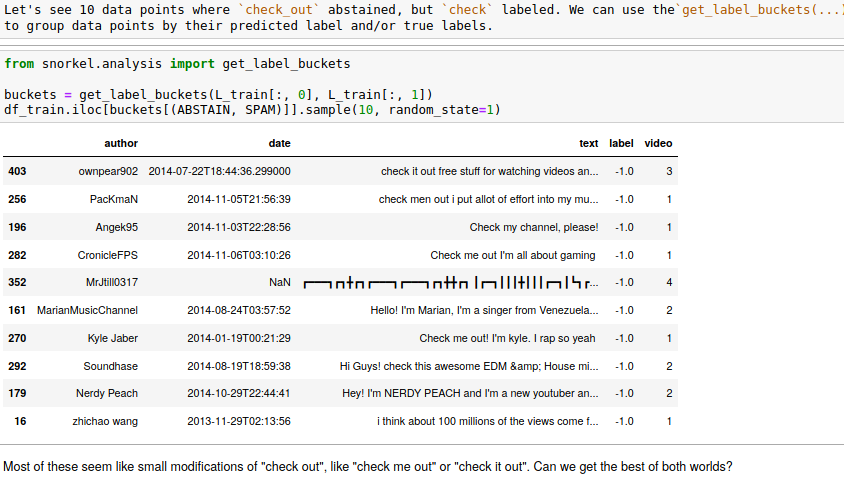
\includegraphics[width=\textwidth]{figures/examplelfanalysis2.png}
note: here, check\_out and check are first and second columns of L\_train. 
\end{frame}

\begin{frame}[fragile]{Okay, now what?}
Once you do this analysis, you can just apply your final LFs list to generate a vector of labeled function outputs for each data point, using LFApplier from few slides before.
\small
\begin{verbatim}
applier = PandasLFApplier(lfs=lfs)
L_train = applier.apply(df=df_train)
L_test = applier.apply(df=df_test)
\end{verbatim}
\end{frame}

\begin{frame}{}
    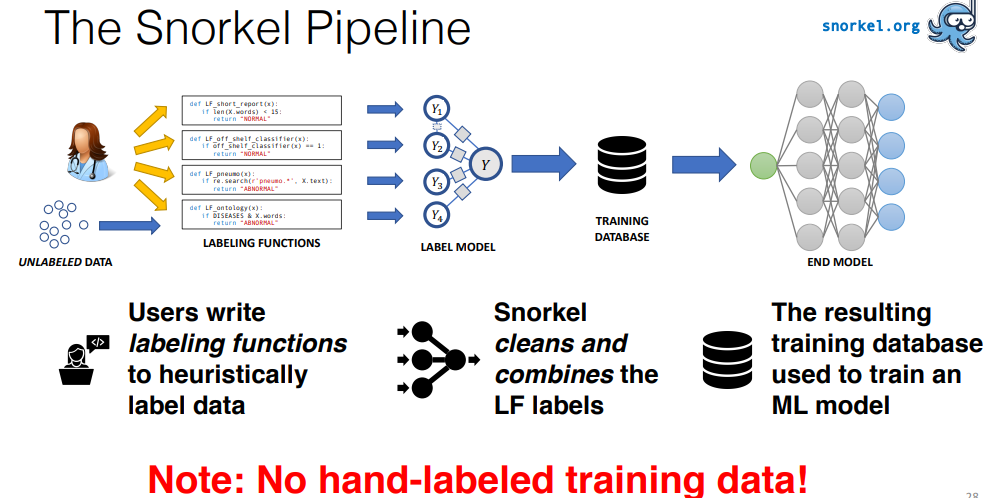
\includegraphics[width=\textwidth]{figures/snorkelradiologyexample.PNG}
    \href{Source}{https://db.cs.washington.edu/events/workshop/2019/slides/alex-ratner.pdf}
\end{frame}

\begin{frame}{From a vector of LF decisions to a "Label Model"}
    \begin{itemize}
        \item Our goal is now to convert the labels from all our LFs into a single noise-aware probabilistic (or confidence-weighted) label per data point. \pause
        \item A simple baseline for doing this is to take the majority vote on a per-data point basis: if more LFs voted SPAM than HAM, label it SPAM (and vice versa). We can test this with the MajorityLabelVoter baseline model. \pause
        \item However, not all LFs are born equal. They all have different coverages, accuracies etc. 
        \item Snorkel has a sophisticated LabelModel, which learns to produce a single set of noise-aware training labels, which are probabilistic or confidence-weighted labels. (\href{https://arxiv.org/abs/1810.02840}{Algorithm paper})
    \end{itemize}
\end{frame}

\begin{frame}{Label Model}
    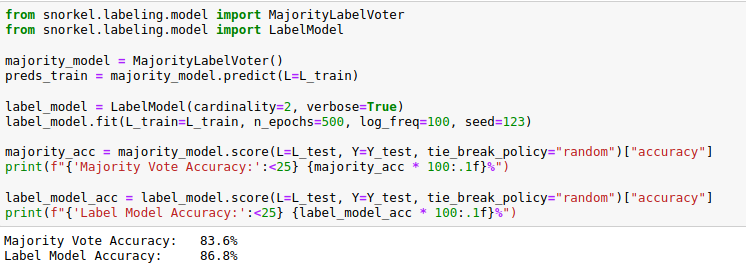
\includegraphics[width=\textwidth]{figures/labelmodel.png}
    Great. Are we done? Why? Why not? 
    
    \pause We eventually want a model that does not need us to rely on LFs perpetually. We are also using LFs to only build this dataset. So, we use this Label Model as input to a "regular" classifier, 
\end{frame} 

\begin{frame}{}
    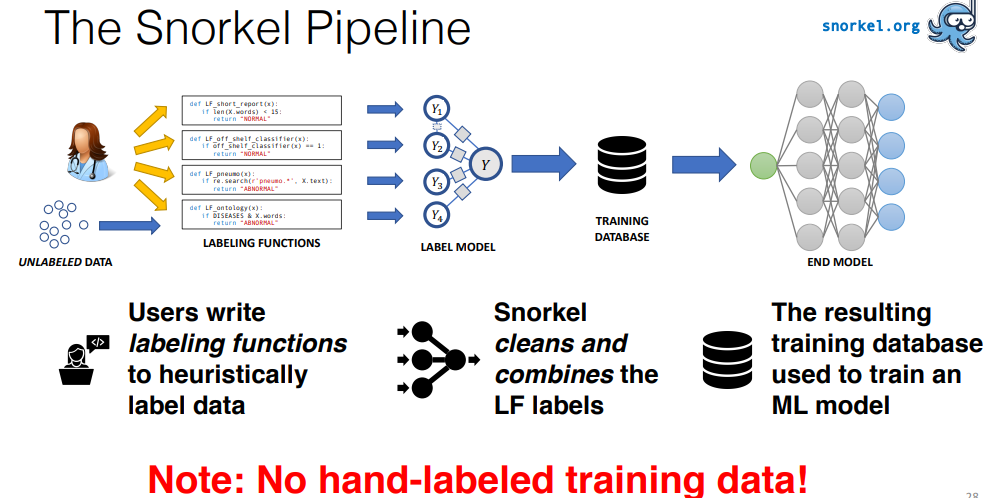
\includegraphics[width=\textwidth]{figures/snorkelradiologyexample.PNG}
    \href{Source}{https://db.cs.washington.edu/events/workshop/2019/slides/alex-ratner.pdf}
\end{frame}

\begin{frame}{Filter out unlabeled datapoints}
    Since we wrote our LFs only based on observation, there may be some data points just not covered by any LF. These are not useful for "learning". They can be removed with snorkel's built in functions: (or we can add LFs to cover these!)
    
    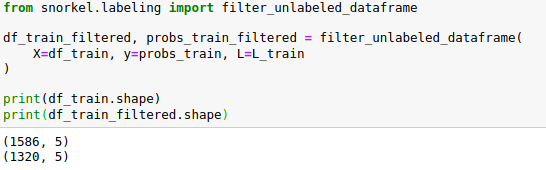
\includegraphics[width=\textwidth]{figures/filteroutunlabeled.png}

    Looks like we lost about 250/1600 data points because of not concentrating much on LFs. 
\end{frame}

\begin{frame}{All set to train again!}
    \begin{itemize}
        \item Now, we have our "labeled" training data. Let us see how we do. How can we know?
   \pause   \item Remember that we have a labeled test data. We can always compare our model performance on that!
   \item In real-world scenarios without dataset, it is still necessary to create a small test set with annotations/labels (following any method we discussed last week - from crowd sourcing to active learning!)
    \end{itemize}
\end{frame}

\begin{frame}{Training a Classifier: Feature Extraction}
    Let us take simple bag of ngrams features for now.
    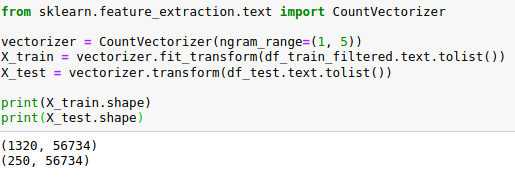
\includegraphics[width=\textwidth]{figures/simplefeaturerep.png}
    
    Note: There are several things I am not doing here e.g., removing stop words, or lower casing etc. 
\end{frame}

\begin{frame}[fragile]{before going ahead with building a model}
    \begin{itemize}
    \item Remember that the label model gives out probabilistic labels (i.e., label distribution instead of one label). 
    \item While there are classifiers that work with that format, many classifier algorithms expect one label.
    \item We can just use the class that got maximum probability from this distribution, using existing function in snorkel.
    \tiny
    \begin{verbatim}
        from snorkel.utils import probs_to_preds
        preds_train_filtered = probs_to_preds(probs=probs_train_filtered)
    \end{verbatim}
    \end{itemize}
    Now, we can just use any classifier like in the sentiment classification example from NLP Pipeline session.
\end{frame}

\begin{frame}{Classification Performance}
        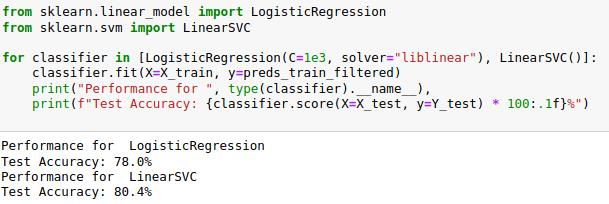
\includegraphics[width=\textwidth]{figures/snorkelspamclassifier.png}
        So, wait ... didn't the LabelModel/MajorityModel do much better than this?? Why are we doing this? 
\end{frame}

\begin{frame}{Label Model vs Classifier}
    \begin{itemize}
        \item What is the difference?
        \item Why can't we just use that label model itself as a classifier- it seems to be doing some sort of classifciation?
        \item Why am I getting poorer result with the classifier here?
        \item Why can't I just use LFs as features, instead of Bag of Words/ngrams etc?
    \end{itemize}
\end{frame}

\begin{frame}{Is this good show?}
\begin{itemize}
    \item 80\% accuracy doesn't seem that bad to me, since randomly predicting SPAM for everything would have given closer to 50\% accuracy on this dataset. (check the dataset stats!)
    \item However, we know the original labels too in this case. How does this approach compare with that? \pause
            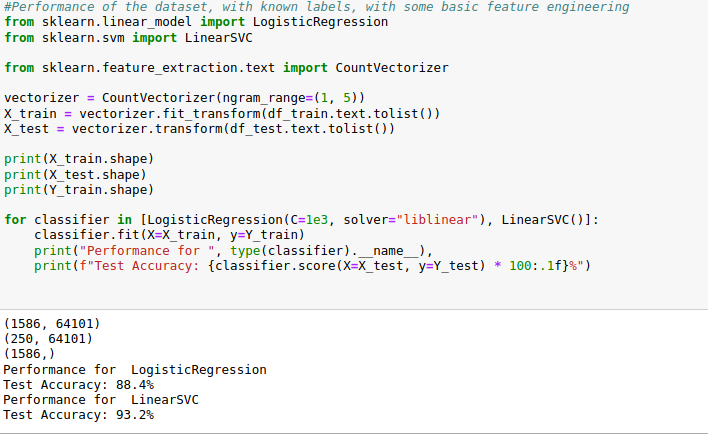
\includegraphics[width=0.7\textwidth]{figures/originalclassifier.png}
\end{itemize}
\end{frame}

\begin{frame}{So why bother about snorkel?}
    \begin{itemize}
        \item Remember, in actual use cases of snorkel, we don't know training labels!
        \item We have to come up with a reasonably good model that does well on test data, WITHOUT labeled training data.
        \item With simple, not so well thought out LFs, we already got 80\% accuracy! May be better LFs will give better results!
    \end{itemize}
\end{frame}

\begin{frame}{Snorkel disclaimer}
        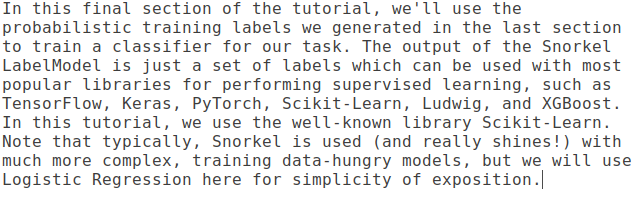
\includegraphics[width=\textwidth]{figures/noteonsnorkel.png}
        
        There is a reason why I chose to show this here, instead of somewhere else during the session. 

\end{frame}

\begin{frame}{}
    \Large Transformation Functions
\end{frame}

\begin{frame}
\frametitle{How to "create" data?}
    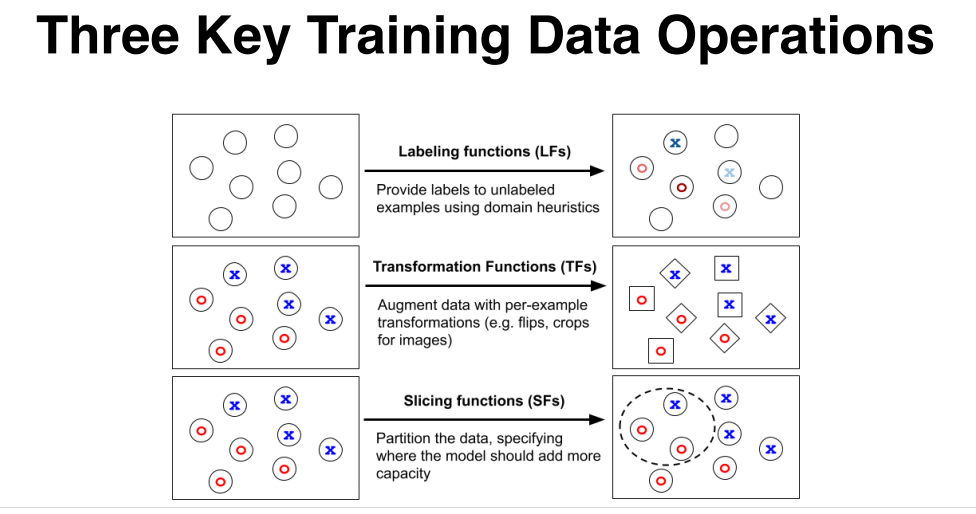
\includegraphics[width=\textwidth]{figures/3snorkelops.PNG}
\end{frame}

\begin{frame}{Data Augmentation}
    \begin{itemize}
        \item Data augmentation is a popular technique for increasing the size of labeled training sets
        \item In this, we create copies of labeled data points. by transforming the text, but preserving the class/category information.
        \item This is very common in work on image classification etc, and quickly becoming popular in NLP too.
    \end{itemize}
\end{frame} %Note, we work with labeled set here!

\begin{frame}{Data Augmentation in Snorkel}
    \begin{itemize}
        \item Accomplished through "Transformation Functions" (@transformation\_function decorator in Python)
        \item Transformation functions are functions that can be applied to a training data point to create another valid training data point of the same class. 
        \item Transformation functions should be atomic e.g. a small rotation of an image, or changing a single word in a sentence. 
        \item We then compose multiple transformation functions when applying them to training data points.
        \item Common ways to augment text includes replacing words with their synonyms, or replacing names entities with other entities. 
        \item Our basic modeling assumption is that applying these operations to a comment generally shouldn't change whether it is SPAM or not.
    \end{itemize}
\end{frame}

\begin{frame}[fragile]{Step 1: Loading the Dataset}
Note: We work with labeled set here! Our goal is different from earlier! (Why?)
\small\begin{verbatim}
df_train, df_test = load_spam_dataset(load_train_labels=True)
Y_train = df_train["label"].values
Y_test = df_test["label"].values
\end{verbatim}
\end{frame}

\begin{frame}{TFs Examples -1}
        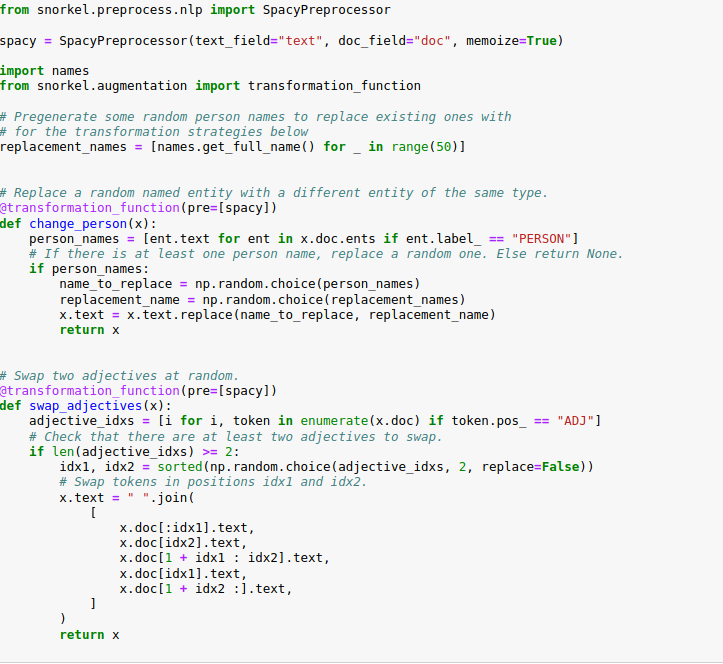
\includegraphics[width=0.8\textwidth]{figures/tfspacy.png}
\end{frame}

\begin{frame}{TFs Examples -2}
        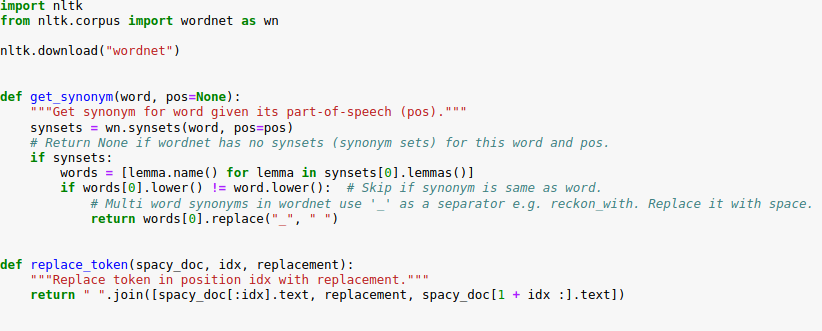
\includegraphics[width=\textwidth]{figures/tfsnltk1.png}
\end{frame}

\begin{frame}{TFs Examples -3}
        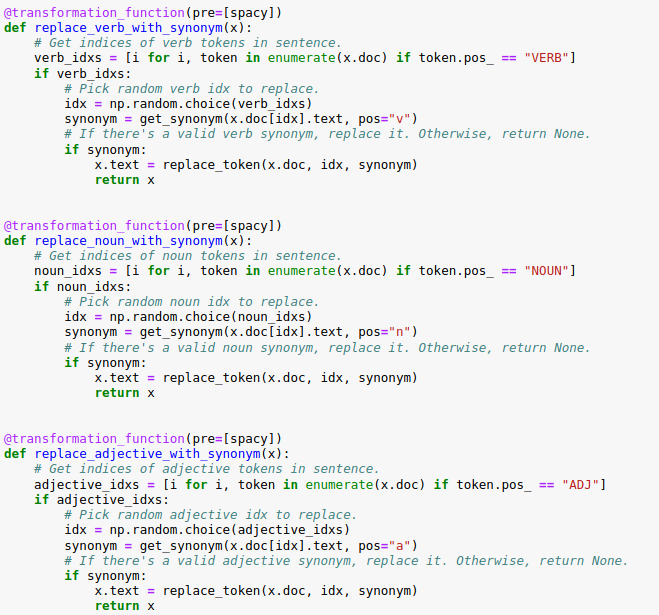
\includegraphics[width=0.8\textwidth]{figures/tfsnltk2.png}
\end{frame}

\begin{frame}{TFs Result}
        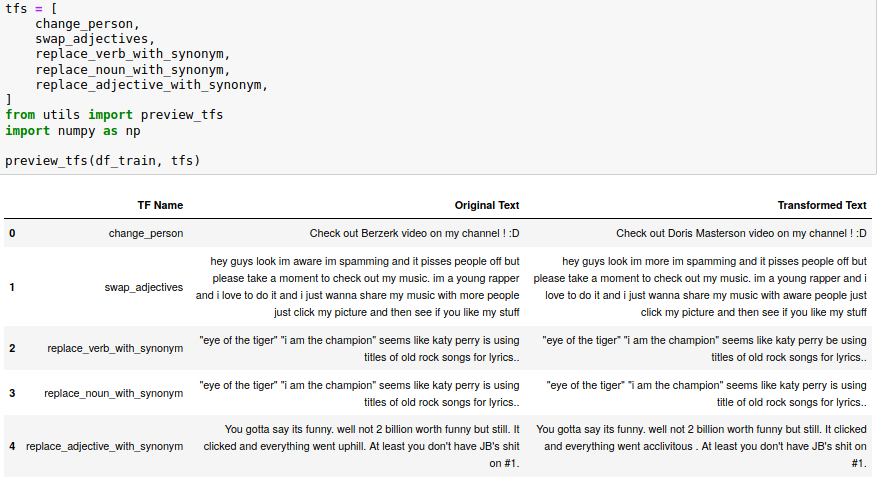
\includegraphics[width=\textwidth]{figures/tfsresult.png}
\end{frame}

\begin{frame}{Notes on TFs}
\begin{itemize}
\item We notice that some changes are trivial.
\item Sometimes they introduce incorrect grammar to the sentence (e.g. swap\_adjectives swapping "young" and "more" above). \pause
\item This can still be helpful for training our model, because it teaches the model to be invariant to such small changes. \pause
\item The TFs are expected to be heuristic strategies that indeed preserve the class most of the time, but don't need to be perfect. 
\item Snorkel is built to work with such noisy output
\end{itemize}
\end{frame}

\begin{frame}{Before Applying TFs on our dataset}
    \begin{itemize}
        \item There are so many of these. Should we apply everything on all data points? Is that necessary? Is it useful? \pause
        \item Snorkel has some data augmentation policies to choose from.
        \item RandomPolicy: Samples sequences of TF indices a specified length at random from the total number of TFs.
        \item MeanFieldPolicy: When we know some TFs are important/useful than others. 
    \end{itemize}
\end{frame}

\begin{frame}[fragile]{TFs policies}
    \small
    \begin{verbatim}
    from snorkel.augmentation import RandomPolicy
    random_policy = RandomPolicy(len(tfs), sequence_length=2, 
                    n_per_original=2, keep_original=True)

    from snorkel.augmentation import MeanFieldPolicy

    mean_field_policy = MeanFieldPolicy(len(tfs),
                        sequence_length=2,
                        n_per_original=2,
                        keep_original=True,
                        p=[0.05, 0.05, 0.3, 0.3, 0.3],)
    \end{verbatim}
\end{frame}

\begin{frame}{Applying TFs}
         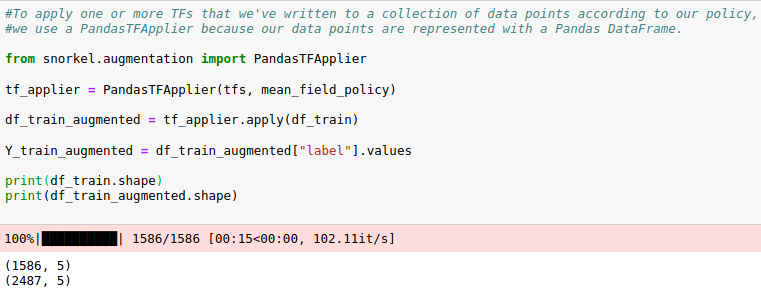
\includegraphics[width=\textwidth]{figures/applyingtfs.png}
         So we almost doubled the size of our dataset.
\end{frame}

\begin{frame}{Training the classifier}
             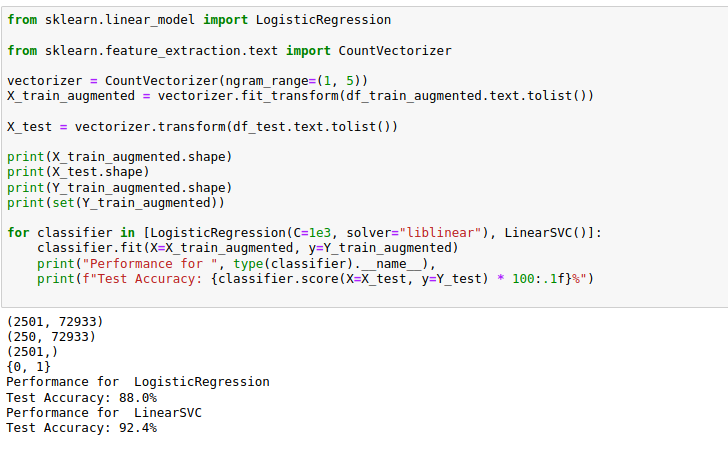
\includegraphics[width=\textwidth]{figures/tfsclassifier.png}
\end{frame}

\begin{frame}{How was it before data augmentation?}
            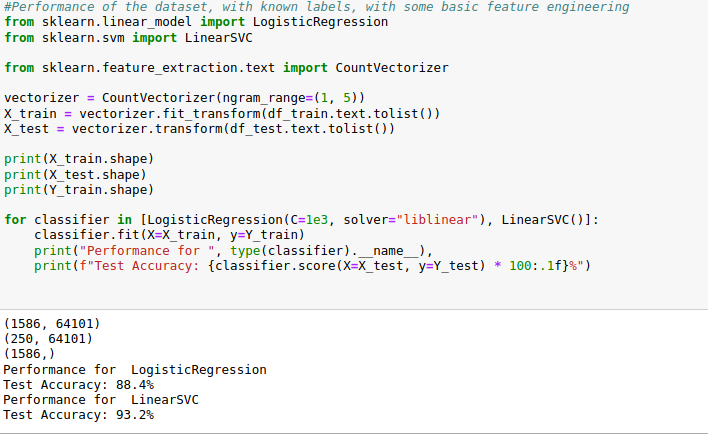
\includegraphics[width=\textwidth]{figures/originalclassifier.png}
\end{frame}

\begin{frame}{Whaat?}
  \begin{itemize}
  \item All this work just to get a slight drop in performance compared to original?? (yeah, I know.. that sucks..)
  \item But the original snorkel tutorial shows a 5\% increase due to data augmentation!! (they directly trained a neural model, and it was bad to start with, so augmentation made it better).
  \item What does that tell you?:  \pause
  \begin{itemize}
      \item We don't have to jump to neural networks right away - there may be *simpler/lighter* solutions that work equally well or better.
      \item Data augmentation is not guaranteed to solve all your model performance problems!
  \end{itemize}
  \end{itemize}
\end{frame}

\begin{frame}{Assignment 2 Description}
\begin{itemize}
    \item 1 question, 15\% of the grade.
    \item Write a rule based NLP system that creates a small corpus of sentences indicating birth/death information of people from Wikipedia biography pages (from the text, not from the info box on the right!) such as place/year of birth/death. 
    \item You can use any language (human/programming).
    \item You can take a look at \href{https://www.snorkel.org/use-cases/spouse-demo}{information extraction tutorial on snorkel} for ideas. 
    \item Write a report describing your approach, how much data you collected etc., and submit along with code. 
\end{itemize}
\end{frame}

\begin{frame}{Next Class}
    \begin{itemize}
        \item Different kinds of neural text embeddings in NLP
        \item How can we use them for NLP
        \item How can we use them for fine tuning
        \item To Do for you: group presentation prep, going through class materials and asking questions on forum. 
    \end{itemize}
    Again, I will upload today's code in a day or two after cleaning it up. 
\end{frame}

\end{document}
